\section{Descripción de los Datos}

Se cuenta con un \textit{dataset}, obtenido de \href{https://www.kaggle.com/rtatman/188-million-us-wildfires}{Kaggle}, con más de 1.88 millones de incendios históricos ocurridos en Estados Unidos, entre 1992 y 2015. La información original se obtuvo a partir del \textit{U.S. Department of Agriculture} \cite{FPA}.

El \textit{dataset} posee 45 columnas, de las cuales ocuparemos aquellas que estén relacionadas con la fecha (como la hora y fecha estimada en que se inició el incendio y el momento en que se controló), con la geografía (como las siglas del estado en que se originó el incendio, y la latitud y longitud del incendio), el tamaño del incendio y la descripción de la causa del incendio (que es la variable objetivo a predecir). 

El resto de variables no representan información relevante para predecir las causas de un incendio. Por ejemplo, el ID del incendio, o del departamento que logró controlar el incendió, no aporta información relevante a la causa del incendio (es más, puede resultar en un sesgo a la hora de predecir).

Se describirán brevemente las columnas que ocuparemos:
\begin{enumerate}
    \item \textit{\textbf{FIRE\_YEAR}}: Corresponde al año en que se originó el incendio.Es una variable temporal.
    \item \textit{\textbf{DISCOVERY\_DATE}}: Es la fecha (aproximada) en que se originó el incendio. Es una variable temporal que, inicialmente, es del tipo float.
    \item \textit{\textbf{DISCOVERY\_TIME}}: Es la hora (aproximada) en que se originó el incendio. Es una variable temporal que, inicialmente, es de tipo cadena.
    \item \textit{\textbf{STAT\_CAUSE\_DESCR}}: Es la causa que originó el incendio. Es una variable categórica de tipo cadena
    \item \textit{\textbf{CONT\_DATE}}: Es la fecha en que se logró extinguir el incendio. Es una variable temporal que, inicialmente, es del tipo float.
    \item \textit{\textbf{CONT\_TIME}}: Es la hora en que se logró extinguir el incendio. Es una variable temporal que, inicialmente, es de tipo cadena.
    \item \textit{\textbf{FIRE\_SIZE}}: Es la extensión (área) que tuvo el incendio (medido en Acres). Es una variable numérica.
    \item \textit{\textbf{FIRE\_SIZE\_CLASS}}: Es una clasificación que utilizan los bomberos para describir la extensión del incendio. Es una variable categórica.
    \item \textit{\textbf{LATITUDE}}: Es la latitud del incendio. Es una variable numérica.
    \item \textit{\textbf{LONGITUDE}}: Es la longitud del incendio. Es una variable numérica.
    \item \textit{\textbf{STATE}}: Es el estado en que se originó el incendio. Es una variable categórica.
\end{enumerate}

Dentro de las columnas mencionadas anteriormente, la columna objetivo será \textit{\textbf{STAT\_CAUSE\_DESCR}}. Las categorías que posee son:
\begin{itemize}
    \item \textbf{Miscellaneous}: Misceláneo.
    \item \textbf{Children}: Causado por infantes.
    \item \textbf{Lightning}: Causado por un rayo.
    \item \textbf{Smoking}: Causado por un cigarro mal apagado.
    \item \textbf{Arson}: Causado con fines maliciosos.
    \item \textbf{Equipment Use}
    \item \textbf{Debris Burning}: Causado por quema de escombros.
    \item \textbf{Campfire}: Causado por un campamento.
    \item \textbf{Railroad}: Causado por un ferrocarril.
    \item \textbf{Missing/Undefined}: Que tiene datos faltantes o que no están definidos.
    \item \textbf{Powerline}: Causado por la linea eléctrica.
    \item \textbf{Fireworks}: Causado por fuegos artificiales.
    \item \textbf{Structure}: Causado por Estructura.
\end{itemize}

Cabe destacar que en la documentación no aparece específicamente una descripción específica de las categorías. Con lo que, varias de estas causas fueron inferidas.

\section{Tratamiento de los Datos}
\subsection{Primer acercamiento de los datos}
En un primer acercamiento de los datos, se observo que existen 3535 filas duplicadas, los cuales se eliminan. 

También, se observa que existen filas con valores nulos; específicamente, en las columnas \textit{\textbf{DISCOVERY\_TIME}}, \textit{\textbf{CONT\_DATE}} y \textit{\textbf{CONT\_DATE}}, siendo aproximadamente la mitad de las filas que poseen valores nulos. Estas filas se eliminan dada la gran cantidad de datos que posee el \textit{dataset}. 

Después de esta limpieza preliminar de los datos, el \textit{dataset} queda con un total de 890821 datos en total (aproximadamente la mitad del dataset original).

\subsection{Tratamiento de las columnas de fecha y hora}
Tratando las columnas temporales, se puede observar que las fechas están en formato de fecha juliana\footnote{Esto corresponde al número de días transcurridos desde el mediodía del 1° de enero del año 4713 a. C.} y el tiempo está representado en formato cadena, con el patrón ``HHMM'', donde HH corresponde a las horas del día y MM corresponde a los minutos. 

Para tratar con estos formatos, primero se transforma las fechas en formato gregoriano, y las horas se transforman en un formato más estándar, digamos, ``HH:MM:SS'', con SS los segundos. Paso seguido, se utiliza la fecha y la hora para transforlas en datos del tipo \textit{DateTime}. Esto se realiza para las columnas de sufijo \textit{\textbf{DISCOVERY\_*}} y \textit{\textbf{CONT\_*}}. De esta forma, 4 de las columnas que se tenían anteriormente, se resumen en dos columnas.

\subsection{Creación de nuevas columnas}
A partir de las nuevas columnas creadas, se crean columnas que entregue la información del mes del incendio (enero, febrero, marzo...), del día de la semana del incendio (lunes, martes...) y la hora del descubrimiento (esto es, si ocurrió a las 8, a las 13, etc...). Esto se hace tanto para la fecha de descubrimiento como la fecha en que se controló el incendio. Además, también se crea una nueva columna que informe el tiempo total en que se logró controlar el incendio. 

Finalmente, se ordena el \textit{dataset} con respecto a la fecha en que se descubrió.

\subsection{Creación de nuevas categorías}\label{subsec:nuevas-cats}
Más adelante se observará que existen categorías bastante mayoritarias frente a otras. Para solucionar este problema, se propondrá una recategorización, que consiste en hacer 4 nuevas categorías:
\begin{itemize}
    \item \textbf{Natural}: Causas naturales. \textit{Lightning} entra en esta categoría.
    \item \textbf{Malicious}: Causas maliciosas. \textit{Arson} entra en esta categoría.
    \item \textbf{Other}: Causas que no se especifican bien. \textbf{Miscellaneous} y \textbf{Missing/Undefined} entran en esta categoría
    \item \textbf{Human}: Hecha por causas humanas, y que probablemente fueron accidente. El resto de clases entran en esta categoría.
\end{itemize}

\section{Análisis Exploratorio de los Datos}
La primera pregunta que alguien se puede realizar es: ¿Cómo están distribuidos el número de incendios con respecto a la causa del incendio? Para responder a la interrogante, se procede a graficar el número de incendios con respecto a sus causas. El resultado del gráfico se puede observar en la Fig. \ref{fig:SCD}. 

\begin{figure}
    \centering
    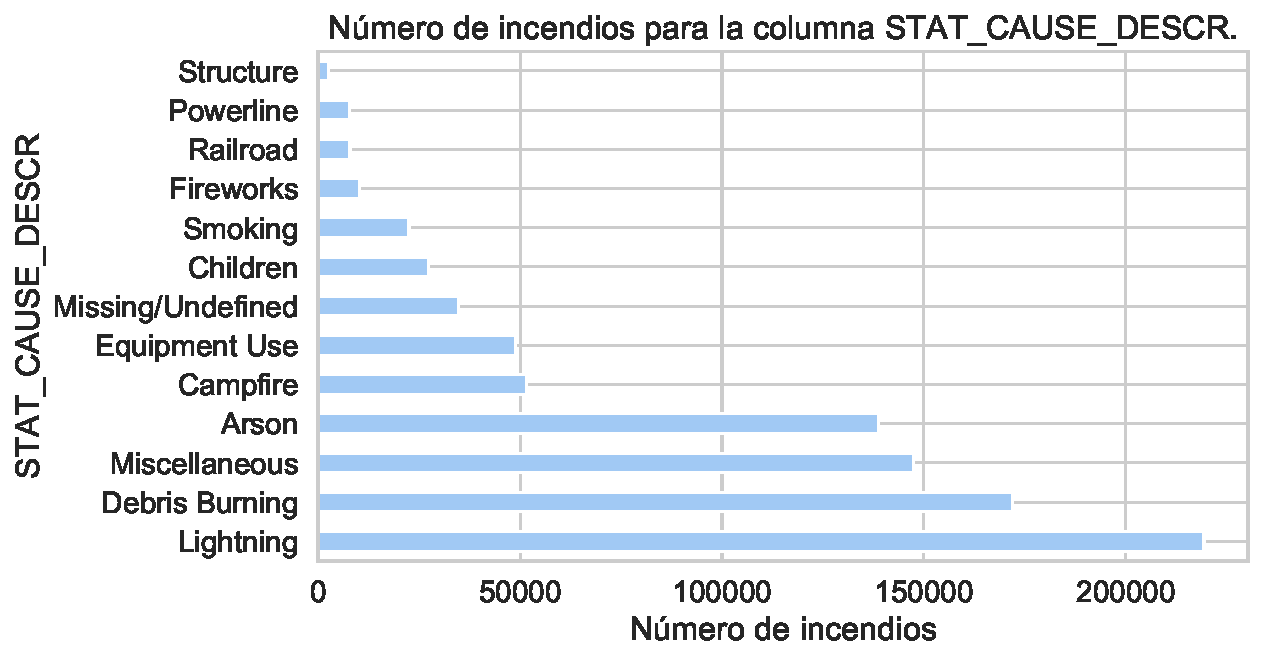
\includegraphics[width=0.48\textwidth]{imagenes/barh_STAT_CAUSE_DESCR.pdf}
    \caption{Gráfico de Causas vs. Número de incendios.}
    \label{fig:SCD}
\end{figure}

Se puede observar que las principales causas de incendio son producidos por rayos (\textit{Lightning}), quema de escombros (\textit{Debris Burning}), de forma miscelánea (\textit{Miscellaneous}) y por razones maliciosas (\textit{Arson}). Mientras que el resto de causas tienen un papel minoritario. 

También, otra de las primeras observaciones que se pueden rescatar, es que el \textit{dataset} está \textit{desequilibrado} (i.e., que existen clases bastante más númerosas que otras). Esto causará que a la hora de realizar clasificación, las clases con mayor número de incendios (como \textit{Lightning}) queden beneficiadas frente a las clases minoritarias (como \textit{Structure}), resultando en \textit{overfitting}.

Para solucionar este problema, se crearán 4 nuevas categorías, como se explica en \ref{subsec:nuevas-cats}. estas son: \textbf{Natural}, \textbf{Malicious}, \textbf{Other} y \textbf{Human}. Luego, se procede a graficar la nueva distribución, que se puede observar en la Fig. \ref{fig:SCDN}.

\begin{figure}
    \centering
    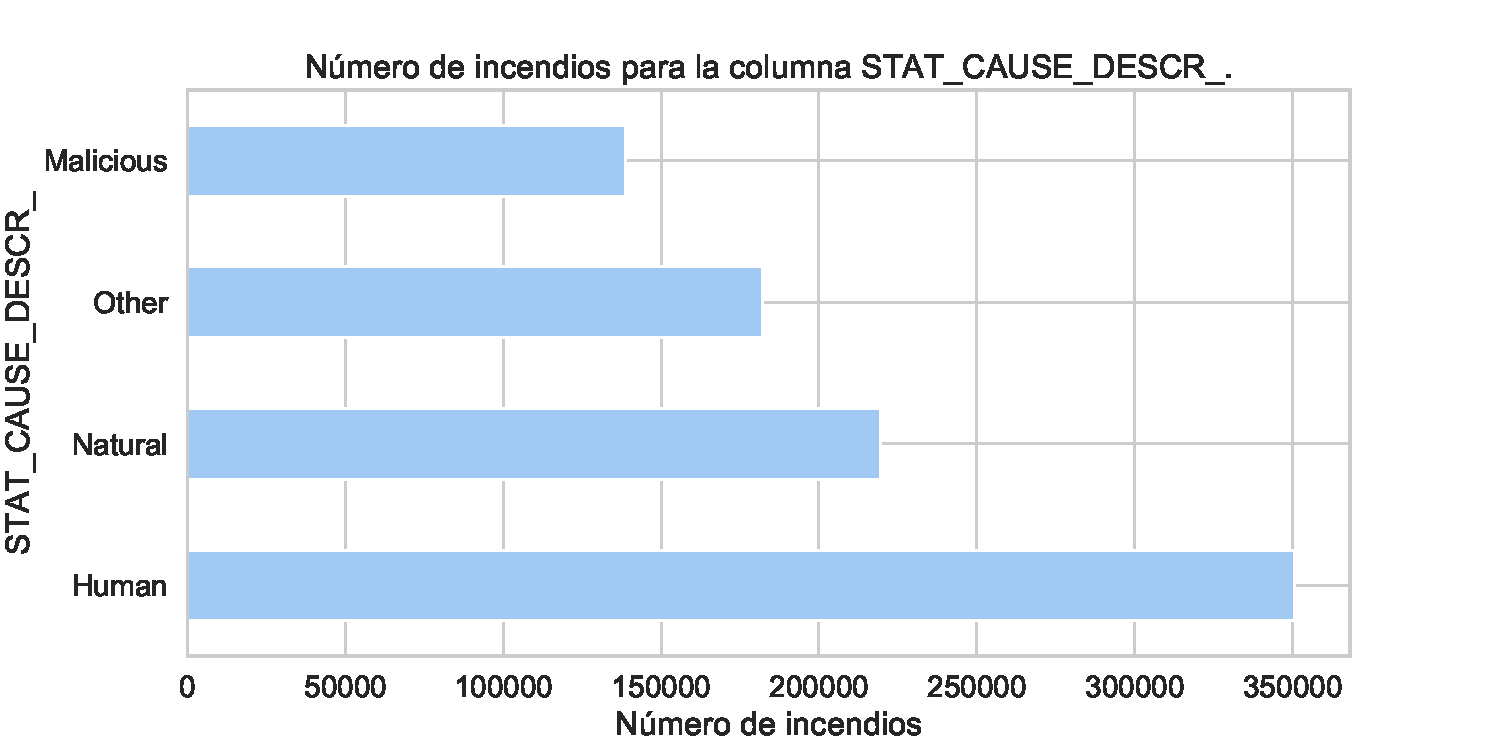
\includegraphics[width=0.48\textwidth]{imagenes/barh_STAT_CAUSE_DESCR_.pdf}
    \caption{Gráfico de Causas Nuevas vs. Número de incendios.}
    \label{fig:SCDN}
\end{figure}

% Incluir la distribución de los datos c/r a los años

% Incluir la distr. de los datos c/r a los años, identificando las categorías

% Incluir la distr. de los datos c/r a los años, identificando las categorías (para la nueva categorización)











% Visualizaciones y resultados relevantes.

% - Análisis exploratorio de datos, mostrar solo visualizaciones y resultados relevantes.
% - Lo realizado para la presentación 1 (que en algunos casos sería lo mismo del análisis exploratorio, o los primeros problemas que tuvieron con sus bases de datos o problemas)
% - Lo realizado para la presentación 2, que sería mostrar en algunos casos el primer experimento que realizaron para resolver su problema, o en otros sería plantear el por qué cambiaron su problema o base de datos.